\chapter{Diseño}
\label{cap:capitulo4}


\vspace{1cm}
El principal objetivo de este TFG es poder desarrollar un comportamiento de navegación autónoma en entornos de simulación 
con el fin de que el dron pueda alcanzar el comportamiento deseado utilizando inteligencia artificial, especificamente redes neuronales
y aprendizaje por refuerzo. Se tomará como entorno de simulación Airsim junto con el motor de videojuegos UnRealEngine, adicionalmente con 
la comunicación de este entorno con AirSim ROS Wrapper Node y Client Airsim, además del estudio y 
análisis de la comunicación entre Airsim, PX4 Autopilot, Mavros y AirSim ROS Wrapper Node .Así, pudiendo evaluar si es posible la unión de Airsim junto con ROS, PX4 y Mavros para
herramientas de diseño en la navegación autonóma de drones. \newline

En primer lugar, en el contexto de la conducción autonóma de drones se evaluará el desarrollo de la percepción mediante redes neuronales y algoritmos de
aprendizaje no supervisado, en especial, clustering y regresiones. 
Posteriormente,el control del UAV se procederá una primera aproximación con un controlador Proporcional Derivativo Integral (PID) desenvolviéndose
en un entorno de carreteras de ambos carriles. \newline

Luego una vez de tener un comportamiento de sigue carril mediante el algoritmo de percepción desarrollado, procederemos a desarollar el algoritmo de 
aprendizaje por refuerzo. Junto con este aprendizaje se realizará análisis de diferentes métricas y resultados
por así entonces de poder encontrar una solución robusta y eficaz al problema que queremos enfrentarnos que será la navegación autónoma de drones en
entornos de carreteras. \newline


\section{Arquitectura}
\label{sec:Arquitectura}

La arquitectura que se ha llevado a cabo en este trabajo se compone de varios elementos fundamentales que se integran entre sí para el desarrollo del seguimiento
del carril. En primer lugar, tendremos un enfoque de simulación Airsim que ofrece la configuración directa de los modelos simulados, ofreciendo la modificación de los sensores
y actuadores disponibles en el entorno de trabajo para obtener los comportamientos deseados. Así de tener una comunicación directa con los componentes intermediarios 
tanto para el control de los actuadores como el manejo de los sensores. Dichos componentes intermediarias se comunican tanto con los programas desarrollados durante en este 
trabajo como con el entorno de simulación para obtener comportamientos de navegación autónoma,facilitando la comunicación entre el entorno de simulación y los programas desarrollados.\newline

Se realizan implementaciones de comportamientos de navegación autónoma basada en redes neuronales y algoritmos de aprendizaje automático, como control clásico basado en 
un controlador Proporcional-Derivativo-Integral así como comportamientos más eficientes y complejos basados en reinforcement learning.

Así junto con el uso de herramientas como PX4 Autopilot y Mavros para así poder analizar la viabilidad junto con el entorno de desarollo Airsim. Las principales implementaciones que se han 
llevado acabo son principalmente dos como se muestra en la figura \ref{fig:infraestructura}:

\begin{enumerate}
  \item \textbf{Seguimiento de carril basado en redes neuronales, algoritmos de aprendizaje automático y control clásico}: Utiliza la red neuronal YOLOP junto con algoritmos de aprendizaje automático para 
   y un control clásico basado en un controlador PID para el seguimiento de carriles.
  \item \textbf{Seguimiento de carril basado en redes neuronales, algoritmos de aprendizaje automático y Q-learning}: tiliza la red neuronal YOLOP junto con algoritmos de aprendizaje automático para 
  con la diferencia de que el control se realiza con un algoritmo de aprendizaje por refuerzo en especial Q-learning para realizar el seguimiento de carriles.
\end{enumerate}

\begin{figure} [H]
    \begin{center}
      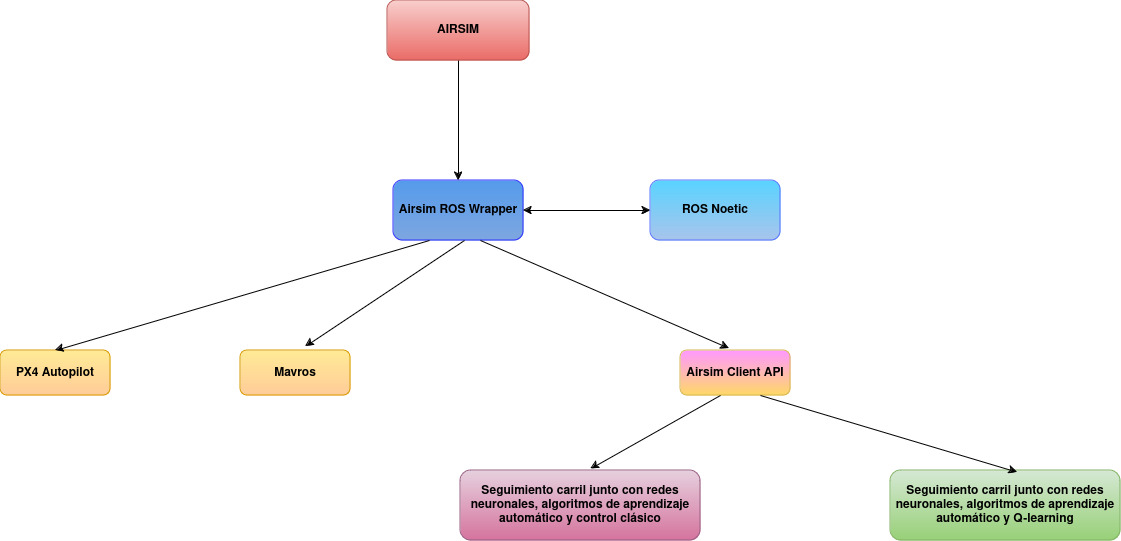
\includegraphics[scale=0.40]{figs/Diseño/Comunicaciones/diagrama-modulos.jpg}
    \end{center}
    \caption{Arquitectura de los componentes utilizados en el TFG}
    \label{fig:infraestructura}
  \end{figure}\

\subsection{Configuración de Integración Distribuida en equipos separados}
En el desarollo de este TFG, hemos tomado la decisión de tener dos enfoques:

\begin{enumerate}
  \item El entorno de simulación Airsim estará en un ordenador con un sistema operativo Windows 10, una gráfica Nvidia RTX 2070 Super con el pluggin de 
  Airsim al cargar el entorno mediante el motor UnRealEngine.
  \item Las plataformas de desarrollo como ROS, Mavros, PX4, QGC y Client Airsim API estarán un  ordenador secundario con un sistema operativo Ubuntu 20.04 con una gráfica Nvidia RTX
  2070.
\end{enumerate}

Esta propuesta fue tomada con la iniciativa de no tener encapsulado en un único componente el entorno de simulación y las plataformas de desarrollo, ya que desembocaba a tener un 
bajo rendimiento en cuanto a velocidad de procesamiento del propio entorno de simulación. La primera aproximación se llegó a construir un entorno de desarrollo con un único ordenador con una grafica
de Nvidia RTX 2070 compuesto de un sistema operativo Linux en donde se integraba el simulador Airsim junto UnrealEngine y las plataformas de desarrollo, obteniendo una media de 60 FPS (Fotogramas por segundo)
conllevando así a tener un compotamiento lento debido a la carga de procesamiento por parte del entorno de simulación. Por causa de Airsim, esta contruido sobre un motor de videojuegos, maximizando los controladores
de gráficos de NVIDIA, lo que puede afectar el rendimiento en sistemas menos optimizados. Por otro lado, si utilizamos un sistema operativo como Windows, es posible lograr un alto rendimiento debido a que Windows
tiende a asignar más recursos a las aplicaciones gráficas junto con la gráfica Nvidia, lo que puede llegar a beneficiar a Airsim. Al tener Airsim en Windows llegamos tener una media 285 FPS siendo
mucho más considerable que la primera opción con un sistema operativo Linux lo cual hace interesante tener Airsim en un entorno que tenga como sistema operativo como Windows. \newline

Por otra parte, para poder utilizar las herramientas junto con el simulador necesitariamos Linux ya que estas herramientas de desarrollo como ROS funcionan con un sistema como Linux lo cual se necesitaria 
tener 2 sistemas operativos diferentes en un mismo equipo. Como se necesitaba desarrollar una comportamiento robusto, eficiente y en tiempo real para el seguimiento de un carril con un dron se decidió
la separación en dos equipos para así conseguir el mejor rendimiento por ambas partes. \newline

El entorno de simulación Airsim se puede comunicar como hemos mencionado con PX4 y Mavros siguiendo un esquema de comunicaciones marcado por la propia página oficial de 
PX4\footnote{\url{https://docs.px4.io/main/en/simulation/}} como se muestra en la siguiete figura:

\begin{figure} [H]
  \begin{center}
    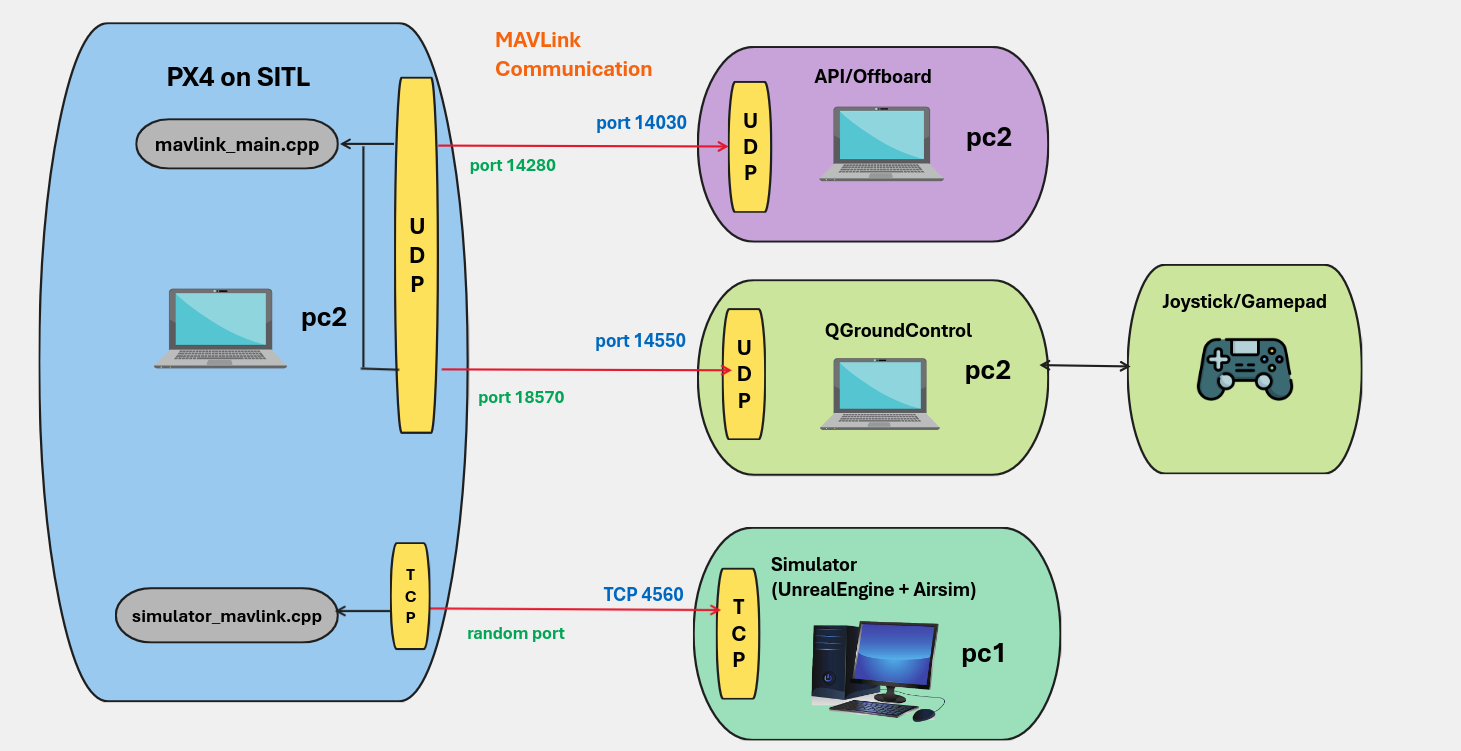
\includegraphics[scale=0.2]{figs/Diseño/Comunicaciones/diagrama_comunicaciones.png}
  \end{center}
  \caption{Diagrama de comunicaciones entre PX4, QGC y Airsim}
  \label{fig:diagramapx4}
\end{figure}\

En donde las comunicaciones internas con PX4 Autopilot se realizan mediante la ejecución del programa px4\_sitl\_default none\_iris y los puertos asignados los realiza la propia
API de Mavlink además de tener la posibilidad con PX4 de comunicarnos con QGC.

\begin{figure} [H]
  \begin{center}
    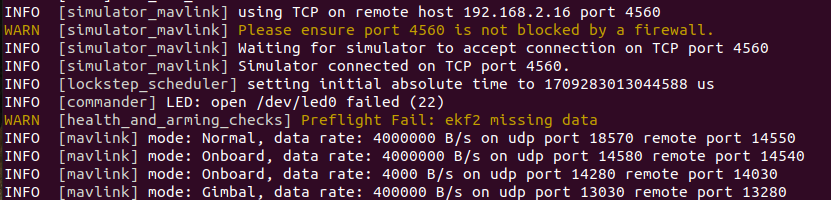
\includegraphics[scale=0.5]{figs/Diseño/Comunicaciones/puertos.png}
  \end{center}
  \caption{Salida de la terminal ejecutando PX4 SITL}
  \label{fig:SalidaTerminal}
\end{figure}\

A lo largo del desarrollo de este trabajo, nos hemos encontrado diferentes difultades respecto a la comunicación directa entre PX4 y el simulador, ya que a menudo cuando se llegaba a 
comunicar las plataformas de desarrollo entre PX4 y Airsim se producian latencias afectando a la sincronización del comportamiento autónomo que queremos desarrollar. Además de que al tener
una capa de comunicación extra con la propia herramienta PX4 Autopilot, Mavros. El acceso no es totalmente directo y puede llegar a ser dificultosopor lo que se optó a utilizar 
Client Airsim por su comunicación directa con el simulador y al estar construida desde la base que se puede llegar acceder directamente al simulador sin llegar a producir capas externas y 
esta pensanda para realizar comportamientos en tiempo real. 

En resumen, la comunicación constará de Airsim ROS Wrapper para acceder a los diferentes sensores como Cámara, Lidar y GPS, Client Airsim para el control del vehículo y el entorno
de simulación Airsim. El diagrama de comunicaciones que se muestra en la figura \ref{fig:diagramadeAirsim} consiste en una sencilla implementación de tener 2 equipos diferentes que
constan del entorno de simulación y de las plataformas en donde iremos desarrollando los diferentes comportamientos como los algoritmos de percepción y control. 

\begin{figure} [H]
  \begin{center}
    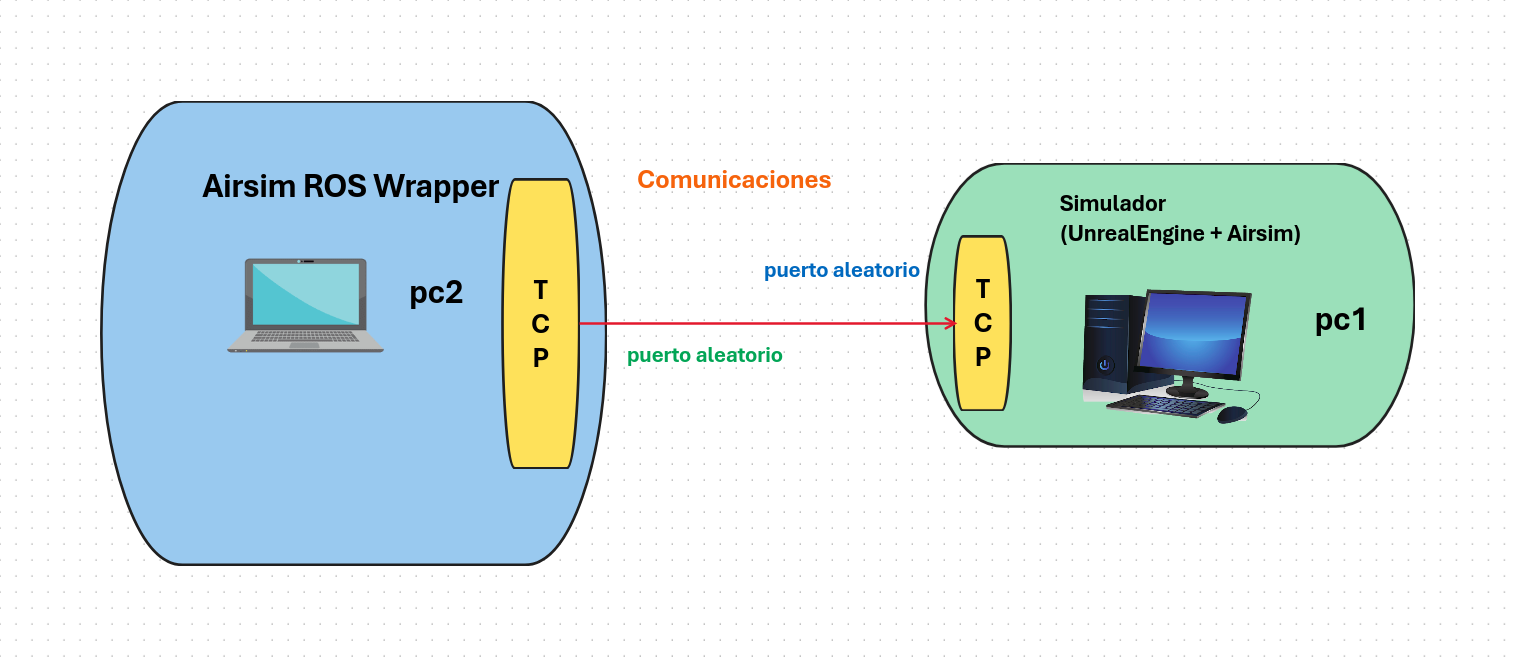
\includegraphics[scale=0.3]{figs/Diseño/Comunicaciones/diagrama_comunicaciones_airsim.png}
  \end{center}
  \caption{Diagrama de comunicaciones}
  \label{fig:diagramadeAirsim}
\end{figure}\

\section{Preparación del entorno de simulación}
\label{sec:Preparación_entorno}

Como mencionamos en la sección \ref{sec:Airsim}, utilizaremos como simulador Airsim junto con el motor UnRealEngine. Para llevar acabo la construcción del entorno, primero tendremos 
que instalar UnrealEngine. Para ello, seguiremos las instrucciones marcadas por la página oficial de Epic Games\footnote{\url{https://www.unrealengine.com/en-US/download}} y trabajaremos con la versión 4.27.2. 

Una vez se tenga UnRealEngine instalado, procederemos a configurar el entorno de simulación que necesitamos, para ello realizaremos la configuración del fichero settings.json con las diferentes
secciones. Por defecto, cuando ejecutamos por primera vez Airsim, el propio simulador nos crea este fichero dentro de una carpeta denonimada Airsim dentro de la carpeta Documentos en Windows, lo cual
es bastante cómodo ya que podemos realizar la modificación de dicho archivo a nuestras necesidades. 


\subsection{Configuración del dron y del entorno}
\label{subsec:Configuración del dron y del entorno}

En primer lugar utilizaremos el entorno de simulación Coastline de los diferentes entornos que nos ofrece Airsim para Windows. Al descargarnos dicha carpeta, contendrá el ejecutable para
poder abrir el entorno con Airsim junto con las carpetas de modelos de simulación, como las carreteras, montañas y plantas. Dentro de estas carpetas, eliminaremos dichos componentes 
de simulación que nos puede dificultar cuando desarrollemos la percepción como plantas y señales de tráfico que se ubican encima de las lineas de detencción del carril ya que esto nos puede perjudicar
en un futuro en la detencción con la red neuronal YOLOP.\newline
Por defecto, la primera vez que ejecutamos un entorno en Airsim, se crea el archivo settings.json en donde se almancenará por defecto en una carpeta 
llamada airsim ubicada en Documentos en Windows. \newline

Cuando tengamos el fichero settings.json creado, ya podremos equipar al vehículo con características como qué sensores utilizará, 
el tipo de vehículo, el tipo de simulación, la comunicación y más. 

\begin{enumerate}
  \item \textbf{SimMode}: Multirotor
  \item \textbf{ClockType}: SteppableClock. Este tipo de reloj permite un control efectivo y manual sobre el avance en el propio simulador, es particularmente útil en simulaciones
  de pruebas donde buscamos un control detallado del tiempo.
  \item \textbf{Vehicles}: En esta sección definiremos las características del vehículo y su comunicación
  \begin{itemize}
    \item \textbf{VehicleType}: SimpleFlight
    \item \textbf{UseSerial}: False
    \item \textbf{ControlIp}: Remote
    \item \textbf{LocalHostIp}: 192.168.2.16
    \item \textbf{Sensors}: Definiremos una pequeña sección de sensores
      \begin{itemize}
        \item \textbf{Lidar}: Definiremos caracteristicas del propio sensor como el tipo, su rango, el número de canales
      \end{itemize}
  \end{itemize}
\end{enumerate}

Si no se define la posición inicial del dron, por defecto el propio simulador te establece el vehiculo en el punto que decida Airsim. 


\begin{figure} [H]
  \begin{center}
    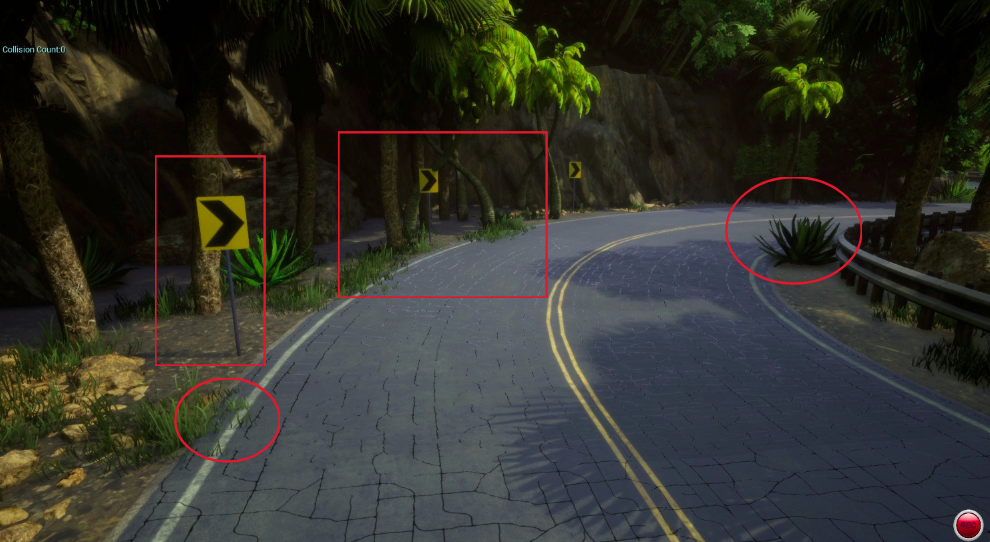
\includegraphics[scale=0.4]{figs/Diseño/coastline3.png}
  \end{center}
  \caption{Visualización del entorno original ilustrando los objetos dificultando la
  percepción de la carretera}
  \label{fig:CoastlineModificado}
\end{figure}\

  \subsection{Instalación de las herramientas de desarrollo}
  \label{subsec:Instalación de las herramientas de desarrollo}
  La instalación de las herramientas de desarrollo se realizarán en el segundo ordenador con el sistema operativo Linux. Constará de las 
  siguientes:
  \begin{enumerate}
    \item \textbf{ROS}: Como se menciona en la documentación oficial de ROS \cite{roswiki} , ROS consta de diferentes conjuntos de paquetes versionados que permiten a los desarrolladores
    trabajar con un código relativamente estable hasta que estén preparados y puedan publicar versiones robustas y eficientes. En nuestro caso, utilizaremos la distribución Noetic\footnote{\url{http://wiki.ros.org/noetic}}
    debido al uso de Airsim debido a que esta distribucion se encuentra siendo una de las más estables para poder trabajar junto con Airsim\footnote{\url{https://microsoft.github.io/AirSim/airsim_ros_pkgs/}}. 

    \begin{figure} [H]
      \begin{center}
        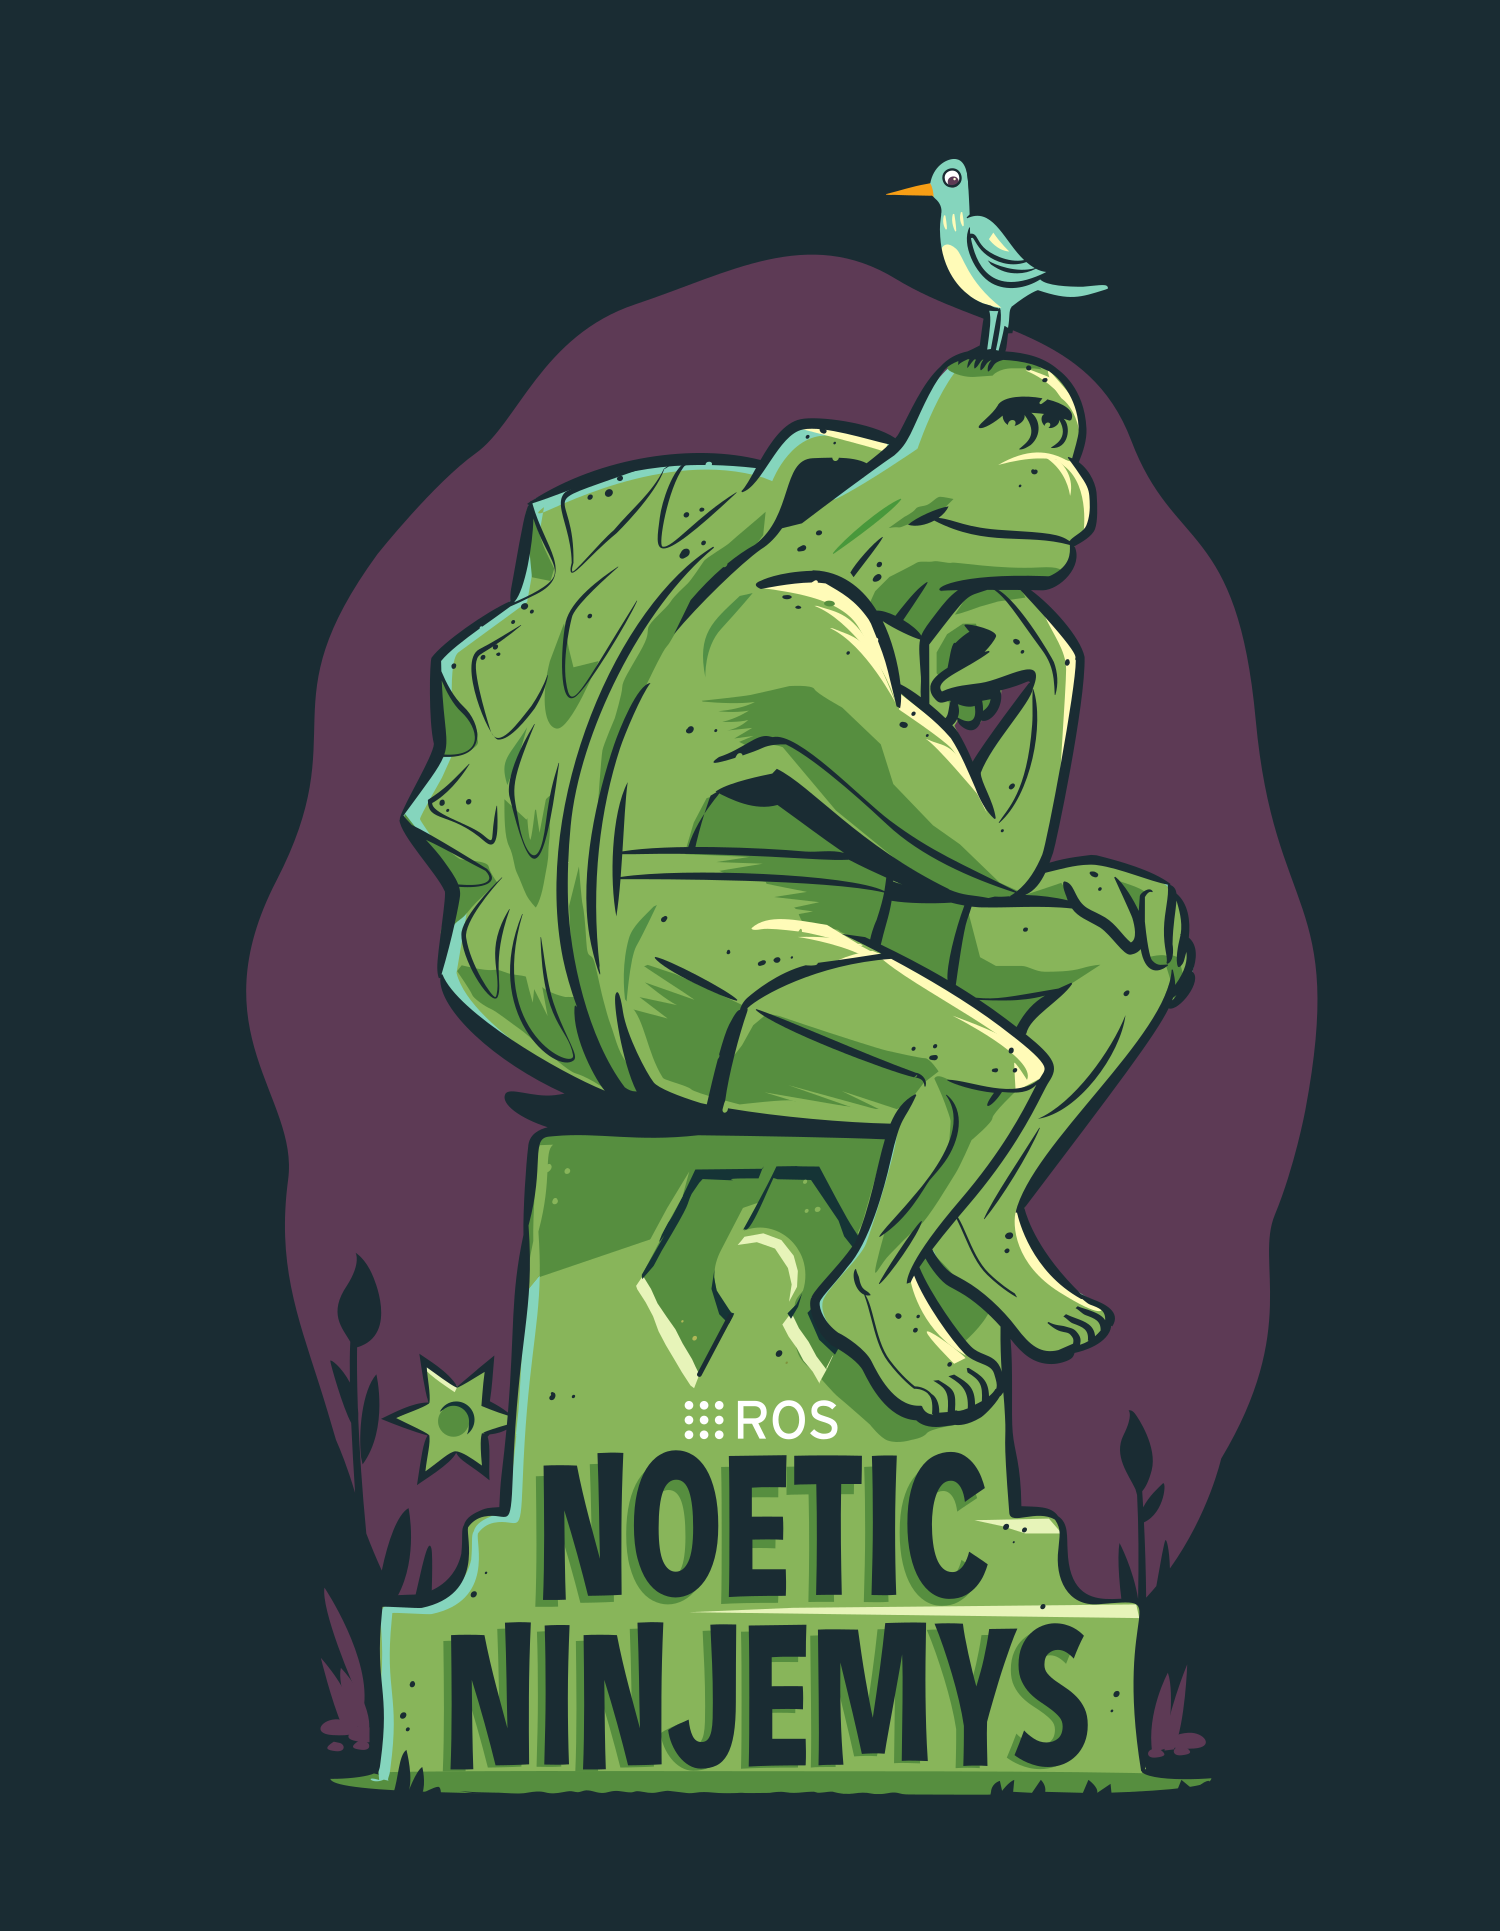
\includegraphics[scale=0.3]{figs/Plataformas_Desarollo/ros-noetic.png}
      \end{center}
      \caption{Logotipo de ROS noetic}
      \label{fig:ROS noetic}
    \end{figure}\
    \item \textbf{Airsim ROS Wrapper}: Descargaremos del repositorio de Airsim a través de su página de github \footnote{\url{https://github.com/microsoft/AirSim}}. \newline
    \begin{lstlisting}
      git clone https://github.com/microsoft/AirSim.git
    \end{lstlisting}
    Cuando tengamos dicho repositorio descargado, lo que realizaremos sera la compilación y configuración de Airsim mediante los scripts build y setup como se pauta en la guía oficial.
    \newline
    Ahora para poder utilizar el Airsim ROS Wrapper que nos proporciona ROS, tendremos que irnos a la carpeta dentro del repositorio de Airsim clonado previamente y buscar la carpeta de ros y construir el paquete 
    mediante el comando \texttt{catkin\_make}. Cuando tengamos realizado dicho paso tendremos que activar el wrapper en el fichero .bashrc de Linux mediante la siguiente linea:\newline

    \begin{lstlisting}
      source /home/$USER/Airsim/ros/devel/setup.bashrc
    \end{lstlisting}
     siendo \$USER la variable de entorno que contiene el nombre del usuario que actualmente tiene iniciada sesión en el equipo.

     A partir de activar el entorno de trabajo para ros, utilizaremos el nodo AirSim ROS Wrapper Node \ref{sec:wrapper} junto con un launcher airsim\_node.launch proporcionando
     la dirección IP en donde se encuentra Airsim.\newline

     \begin{lstlisting}
      roslaunch airsim_ros_pkgs airsim_node.launch output:=screen host:=192.168.2.16
    \end{lstlisting}

  \end{enumerate}

\section{Percepción}
\label{sec:Percepción}
Para el desarrollo de la percepción una primera aproximación fue utilizar
procedimientos de visión clásica, es decir, procesar la imagen y mediante métodos de la libreria OpenCV
poder detectar las diferentes líneas que pueden haber en la carretera. El problema que nos podemos encontrar que al realizar esta primera proximación, al tener un 
entorno fotorrealista, estos métodos se quedan bastante pobres desembocando una percepción muy poco robusta e ineficiente. Por lo que se optó la utilización
de una red neuronal llamada YOLOP y algoritmos de aprendizaje automático poder construir la percepción. \newline

Para obtener la imagen del entorno, nos subscribiremos al topic /airsim\_node/Drone/front\_center\_custom/Scene que ofrece el nodo AirSim ROS Wrapper Node
 y mediante un método de ROS denonimado CvBridge\footnote{\url{http://wiki.ros.org/cv_bridge}} podremos convertir dicha imagen en formato OpenCV y trabajar con ella a traves de OpenCv.\newline

\subsection{Inferencia de YOLOP}
\label{sec:Inferencia de YOLOP}

Para realizar la deteción de las líneas en la carretera nos ayudaremos de la red neuronal YOLOP\ref{sec:YOLOP}. A continuación hablaremos sobre la inferencia del YOLOP con sus distintos pesos preentrenados. En primer lugar, 
como anteriormente hemos comentado, el archivo End-to-end.pth es un archivo de pesos construido en Pytorch, cuando queremos cargar
dichos pesos con el modelo podemos hacerlo de dos maneras: Podemos realizarlo mediante la CPU o la GPU. 
Para ello, si queremos cargar el modelo de YOLOP con los pesos preentrenados End-to-end.pth se realizará cargando el modelo de la red a través de su repositorio de github \footnote{\url{https://github.com/hustvl/YOLOP}}
especificando el modelo de la red neuronal y la opción 'pretrained' colocada con valor True, diciendo que cargaremos los pesos de formato pytorch del archivo End-to-end.pth.\newline
\begin{code}[h]
  \begin{lstlisting}[language=Python]
  import torch
  
  model = torch.hub.load('hustvl/yolop', 'yolop', pretrained=True)

  \end{lstlisting}
  \caption[Cargar modelo YOLOP con pesos preentrenados End-to-end.pth]{Cargar modelo YOLOP con pesos preentrenados End-to-end.pth}
  \label{cod:codejemplo}
  \end{code}  

Una vez tengamos el modelo cargado del repositorio, podemos escoger si queremos hacer la inferencia en la CPU o GPU, para ello tendremos que especificar como 
lo queremos hacer. En nuestro, elegiremos la opción de GPUp ara realizar la inferencia y le asignaremos al modelo que realizaremos la inferencia por GPU.\newline

  
  \begin{code}[h]
    \begin{lstlisting}[language=Python]
   
    device = torch.device("cuda" if torch.cuda.is_available() else "cpu")
    model = model.to(device)
  
    \end{lstlisting}
    \caption[Cargar modelo YOLOP escogiendo como disposivo la GPU]{Cargar modelo YOLOP escogiendo como disposivo la GPU}
    \label{cod:codeloadYOLOP}
    \end{code}  

    Por último, nos quedaria convertir la imagen en un tensor antes de realizar la inferencia. Para poder realizarlo, utilizaremos la funcion transforms.toTensor\footnote{\url{https://pytorch.org/vision/main/generated/torchvision.transforms.ToTensor.html}} 
    y después añadiremos una dimensión más con unsqueeze(0) , esto se debe 
    a que el modelo de YOLOP espera una entrada específica llamada batch\_size. Batch\_size es el número de imagenes que se procesarán juntas
    (generalmente 1 para inferencia) por lo que el tensor tendrá esta forma: (batch\_size, channels, height, width)\newline

    \begin{code}[h]
      \begin{lstlisting}[language=Python]
     
        from torchvision import transforms

        transform = transforms.ToTensor() 
                    
      imagen_tensor = transform(cv_image).to(device).unsqueeze(0)
      _, da_seg_out, ll_seg_out = self.model(imagen_tensor)
    
      \end{lstlisting}
      \caption[Inferencia del modelo]{Inferencia del modelo en Pytorch}
      \label{cod:codejemplo}
      \end{code}  

    \newpage
    Como resultado de la inferencia obtendremos un tensor de salida que corresponde la probabilidad de detencción de la segmentación
    de la calzada y la detencciñon de las lineas de la calzada. Dicho tensor habrá que convertirlo en una imagen para poder visualizar
    dicho resultado como una imagen. 
    Por ello, convertiremos el tensor en un array numpy y realizaremos una transformacion para cambiar las dimensiones de (H,W,C) 
    a (C,H,W) esto se realiza ya que en Opencv representa imagenes en formato Numpy array y se transpone las dimensiones porque las
    imagenes de Opencv tiene la forma de (H, W, C)\footnote{\url{https://lindevs.com/convert-pytorch-tensor-to-opencv-image-using-python}}. 
    \newline

    Obtendremos un array de Numpy que normalizaremos con valores de 0-1.La normalización 
    ayudar a igualar la escala de los pixeles de la imagen. Finalmente se podrá mostrar el resultado de la inferencia de la red 
    en una imagen. Al normalizar los valores de 0-1, los pixeles con un valor 1 se mostrarán en la imagen final, asignándoles un color
    para visualiza el resultado de la segmentación de la calzada y de la detencción de las lineas de la calzada. \newline
    \newpage
    \begin{code}[h]
      \begin{lstlisting}[language=Python]
        import cv2
        import numpy as np
        for image in (da_seg_out,ll_seg_out):

          image_np = image.detach().cpu().numpy()
          image_array = np.transpose(image_np, (2, 3, 1, 0))

        
          image_norm = cv2.normalize(image_array[:,:,1,:], None, 0,1, cv2.NORM_MINMAX, cv2.CV_8U)

          images.append(image_norm)

    
        cv_image[images[0] == 1] = [0, 255, 0]
        cv_image[images[1] == 1] = [0, 0, 255]

        cv2.imshow('Image', cv_image)
        cv2.waitKey(1)

    
      \end{lstlisting}
      \caption[Resultado de la inferencia del modelo YOLOP]{Resultado de la inferencia del modelo YOLOP}
      \label{cod:codejemplo}
      \end{code}  

      Para poder utilizar los pesos preentrenados de Onnx, tendremos que realizar la configuración de los drivers de CUDA con la versión disponible para Onnx Runtime, 
      dichas versiones tienen que ser compatible entre si mismas. Para ello nos guiaremos por la tabla requisitos de la página oficial de Onnx Runtime\footnote{\url{https://onnxruntime.ai/docs/execution-providers/CUDA-ExecutionProvider.html}}. \newline

      Cuando tengamos todo preparado y configurado ya podremos realizar los pasos de la inferencia con los pesos preentrenados de Onnx. En primer lugar,cargaremos el modelo
      
      \begin{code}[h]
        \begin{lstlisting}[language=Python]
          import onnxruntime as ort

          ROUTE_MODEL = "/home/bb6/YOLOP/weights/yolop-320-320.onnx"
          ort_session = ort.InferenceSession(ROUTE_MODEL,providers=['CUDAExecutionProvider'])
      
        \end{lstlisting}
        \caption[Cargar modelo]{Cargar modelo YOLOP-320-320.onnx}
        \label{cod:codejemplo}
        \end{code}  

        Como se observa en el código 4.5, a la hora de cargar el modelo escogemos como provider CUDAExecutionProvider. Cuando trabajamos con ONNX Runtime, 
        podemos especificar qué proveedores de ejecución utilizar para ejecutar el modelo ONNX que escojamos, cada proveedor contiene un conjunto de núcleos optimizados para un objetivo específico (por ejemplo, CPU, GPU, IoT) y 
        se especifican como una lista en el orden de prioridad. En nuestro caso escogeremos CUDA para ejecutar mediante la GPU. 
        \newline
        A continuación preprocesaremos las imagenes de entrada que le daremos al modelo, al escoger el modelo de yolop-320-320.onnx, las imagenes deben tener una dimensión de 320x320, para ello
        utilizaremos un método implementado por ellos, en el cuál redimensionaremos la imagen como se pide para el modelo. 
        Una vez que tengamos la imagen preparada, daremos comienzo a la inferencia del modelo de yolop-320-320.onnx. \newline
      
        \begin{code}[h]
          \begin{lstlisting}[language=Python]
            _, da_seg_out, ll_seg_out = self.ort_session.run(
              ['det_out', 'drive_area_seg', 'lane_line_seg'],
              input_feed={"images": img}
          )
        
          \end{lstlisting}
          \caption[Inferencia del modelo yolop-320-320.onnx]{Inferencia del modelo yolop-320-320.onnx}
          \label{cod:codejemplo}
          \end{code}  

        La inferencia del resto de modelos de Onnx se realizan de la misma forma pero teniendo en cuenta que se tendrá que cambiar las dimensiones de las imagenes de entrada y la ruta
        en donde se almacena dicho modelo. 


\subsubsection{Resultados de YOLOP }
\label{sec:resultados}
En esta sección contrastaremos los resultados dde los diferentes pesos preentrenados que ofrece la red neuronal YOLOP. Como podemos observar en la figura \ref{fig:pesos_preentrenados} 
mostramos la media en realizar la inferencia de YOLOP utilizando los pesos preentrenados End-to-end.pth, yolop-320-320.onnx,yolop-640-640.onnx e yolop-1280-1280.onnx en segundos.

\begin{figure} [H]
  \begin{center}
    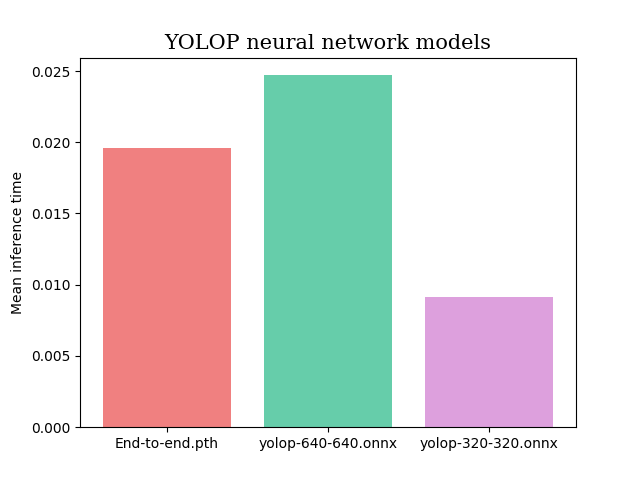
\includegraphics[scale=0.6]{figs/Diseño/Percepcion/Results-Yolop.png}
  \end{center}
  \caption{Resultados de los pesos preentrenados del modelo YOLOP}
  \label{fig:pesos_preentrenados}
\end{figure}\

Como podemos observar en la figura 4.6, los pesos preentrenados que tiene una inferencia menor al resto se trata de yolop-320-320.onnx, tiene un tiempo de inferencia alrededor de 0.010s, esto
significa que el modelo YOLOP con estos pesos tiene aproximadamente un rate de 100 FPS. Si comparamos este resultado con los restantes pesos, es el ganador en cuanto 
en tiempo de inferencia, rate y mejores resultados. 
Onnx está diseñado para ser más eficiente en términos de memoria y velocidad de inferencia en cuanto Pytorch, lo que puede mejorar la velocidad y la precisión
del modelo, añadiendo de tener una menor resolución en cuanto al tamaño de las imágenes reduciendo la cantidad de información al procesarlas. Aun así, depende de varios factores y según las necesidades, nosostros
buscamos un equilibrio entre velocidad de inferencia y mejores resultados en cuanto a la detencción como se mostraban en los resultados de la red neuronal \ref{f:resultadosYOLOP}. \newline

\begin{figure} [H]
  \begin{center}
    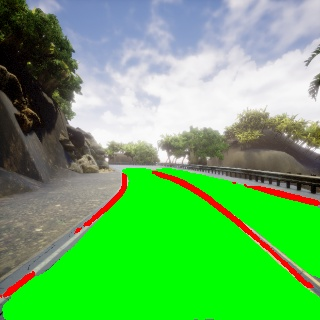
\includegraphics[scale=1.0]{figs/Diseño/YOLOP/onnx-320-320.jpg}
  \end{center}
  \caption{Resultados de los pesos preentrenados yolop320-320.onnx}
  \label{fig:pesos_preentrenados}
\end{figure}\

Una vez escogido el modelo yolop320-320.onnx procederemos a seleccionar las lineas detectadas que nos interesan mediante un algoritmo de aprendizaje no supervisado denonimado clustering.

\subsection{DBSCAN}
\label{sec:DBSCAN}

Para saber con qué lineas detectadas por la red nos quedaremos, utilizaremos un algoritmo de aprendizaje no supervisado llamado clustering, en particular
utilizaremos DBSCAN(Density-Based Spatial Clustering of Applications with Noise)\cite{scikitlearndbscan}.\newline

Dicho algoritmo contiene varios parámetros que son importantes conocerlos y configurarlos: 
\begin{enumerate}
  \item \textbf{Eps}: Consiste en la distancia máxima que puede existir entre dos muestras para que una se considere vecina de la otra. Dicha distancia no se trata de un límite 
  máximo entre las distancias que puede haber dentro de un cluster.
  \item \textbf{Min\_samples}: Es el número mínimo de muestras dentro de un vecindario para que un punto se considere como un punto central incluyendo al propio punto.
  \item \textbf{Metric}: La métrica utilizada para calcular la distancia entre los conjuntos de clústeres (por defecto es la distancia euclidiana). 
\end{enumerate}
Los valores de los parámetros de la distancia máxima y el número mínimo de muestras se deben elegir cuidadosamente, es decir, si colocamos una distancia 
máxima alta puede provocar que los clusters que queramos que pertenezcan a un distinto grupo pertenezcan al mismo grupo. 
Si min\_samples se establece en un valor alto, DBSCAN encontrará clústeres más densos y 
si se establece en un valor bajo, los clústeres encontrados serán más dispersos.
\break
Por lo que para encontrar los valores de estos 2 parámetros fue experimentando y quedandonos con el mejor resultado. En nuestro caso la distancia máxima tendra un valor de 10 
y el número mínimo de muestras sera de 5 muestras. Lo que significa que la distancia máxima que tendrán los puntos para pertenecer al mismo grupo de clústeres sera de 10 de distancia en pixeles
con un mínimo de muestras pertenecientes de 5 muestras. 

Para entender un poco más como funciona el algoritmo, en la siguiente figura recogida por este árticulo\cite{DBSCAN}: 

\begin{figure} [H]
  \begin{center}
    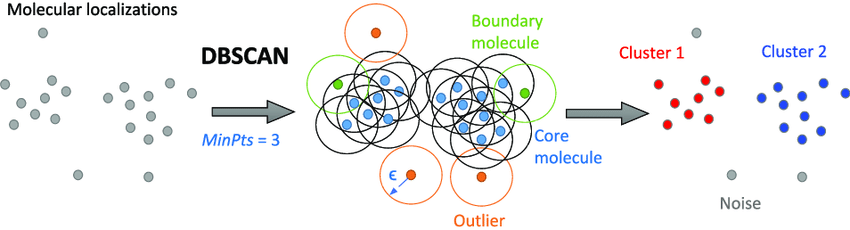
\includegraphics[scale=0.5]{figs/Diseño/DBSCAN/DBSCAN-Illustration.png}
  \end{center}
  \caption{Ejemplo ilustrativo de como funciona el algoritmo de DBSCAN}
  \label{fig:pesos_preentrenados}
\end{figure}\

Se ilustra un ejemplo teniendo un número de muestras ubicadas aproximadamente cercanas unas de otras. Aplicamos el algoritmo de DBSCAN 
teniendo como valor el número mínimo de muestras 3, eso significa que para que se considere una muestra a un grupo de cluster tendrá que tener una densidad de 3. El algoritmo itera por
las muestras y compara el valor de la distancia máxima y el número mínimo de muestras. 
Si ningún de estos dos parámetros no se cumpliese ya que puede darse que una muestra se encuentra lejana del grupo de muestras será etiquetado como ruido, esto quiere decir
que no pertenecerá a ningún grupo de clústeres. Dicho resultado se puede observar en la figura \ref{fig:pesos_preentrenados} como el algoritmo ha catalogado dos grupos de clústeres y 3 muestras
como puntos de ruido. 
\break

Centrandonos en nuestra implementación con el algoritmo de DBSCAN, le pasaremos la imagen de salida de la red neuronal pero con la particularidad que DBSCAN necesitaria que la imagen sea
representada por un array bidimensional de coordenadas x e y de puntos. Para ello utilizaremos la función de Numpy column\_stack\footnote{\url{https://numpy.org/doc/stable/reference/generated/numpy.column_stack.html}} , 
dicha función transforma un array simple de una dimensión a un array de 2 dimensiones, una vez se realice esto obtendremos un array bidimensional para el algoritmo DBSCAN.\newline

\begin{code}[h]
  \begin{lstlisting}[language=Python]
    def clustering(self,cv_image):

    #--Convert image in points
    points_lane = np.column_stack(np.where(cv_image > 0))
    dbscan = DBSCAN(eps=10, min_samples=5,metric="euclidean")
    

    if points_lane.size > 0:
        dbscan.fit(points_lane)
        labels = dbscan.labels_

        # Ignore noise if present
        clusters = set(labels)
        if -1 in clusters:
            clusters.remove(-1)
      
      
            
        for cluster in clusters:
            points_cluster = points_lane[labels==cluster,:]
            centroid = points_cluster.mean(axis=0).astype(int)
            color = self.colors[cluster % len(self.colors)]
            cv_image[points_cluster[:,0], points_cluster[:,1]] = color

        return cv_image
  
  \end{lstlisting}
  \caption[Algoritmo de custering utilizando DBSCAN]{Algoritmo de custering utilizando DBSCAN}
  \label{cod:codejemplo}
  \end{code}  
  

Obtenemos el resultado de DBSCAN con los parámetros configurados de eps = 10 y min\_samples = 5, dicho resultado será una lista con etiquetas de 0 a n, siendo 0 el primer grupo de clusters detectado y 
n el último grupo de clusters detectado. De las listas de etiquetas se eliminarán los clusters que hallan sido etiquetados como ruido, para ello solo basta encontrar la etiqueta con valor -1 ya que
DBSCAN cataloga las muestras ruidosas con -1 y para obtener el resultado solamente bastará iterar en dicha lista y mostrar los puntos correspondientes de cada etiqueta en la imagen de salida

\subsection{Clasificación de clústeres}
\label{clasificación:cluster}
Una vez realizado el algoritmo de DBSCAN necesitamos quedarnos con el grupo de clusters que pertenezcan al carril que queremos seguir, para ello calcularemos los centroides de cada
grupo de clusters detectado y los clasificaremos en función de si se encuentran en la derecha o izquierda de la imagen, es decir, la imagen tiene unas dimensiones de 320x320 por lo tanto 
nos fijaremos en el valor del eje x en el ecuador con valor 160, por lo que cuando calculemos los clústeres serán clasificados en función de los valores de x si se encuentran a la derecha u izquierda de 160 
que es la mitad de la imagen. \newline

\begin{code}[h]
  \begin{lstlisting}[language=Python]
    # Check if the centroid is within the desired lane

    WIDTH = cv_image.shape[1]
    if centroid[1] < WIDTH/2:  # left lane
        left_clusters.append((points_cluster,centroid))
       
    elif centroid[1] >= WIDTH/2:  # right lane
        right_clusters.append((points_cluster, centroid))
       
  
  \end{lstlisting}
  \caption[Clasificación de clústeres según las dimensiones de la imagen ]{Clasificación de clústeres según las dimensiones de la imagen}
  \label{cod:codejemplo}
  \end{code}  


Cuando tengamos clasificado los grupos de los clústeres, necesitamos quedarnos con qué subgrupo de cada grupo de clústeres (izquierda e derecha) nos queremos quedar respecto al carril. Para ello escogeremos dichos grupos mediante una función máximizada
la cual escoge dicho grupo de clusters de la derecha u izquierda en función de la cercania de un punto central P escogido como valor (220,160) siendo 220 el valor de las y e 160 el valor de las x. \newline

Es importante mencionar que cuando trabajamos con puntos en numpy las coordenadas estan opuestas, es decir, en vez de tener el formato (x,y) como estamos acostumbrados a trabajar tienen el formato(y,x). A parte de escoger en función de la cercania de un punto P también esta en función de la densidad de puntos de dicho grupo de clusters de la derecha u izquierda detectados, con
esto conseguimos que no solamente escojamos en función de la cercania si no que también lo haremos según la cantidad de puntos. \newline

\begin{code}[h]
  \begin{lstlisting}[language=Python]
    def score_cluster(self,cluster, center):
      points_cluster, centroid = cluster
    
      proximity = np.linalg.norm(centroid - center)
      density = len(points_cluster)
      return density / proximity

  \end{lstlisting}
  \caption[Función maximizada para escoger el grupo de cluster más cercano y denso respecto al punto P]{Función maximizada para escoger el grupo de cluster más cercano y denso respecto al punto P}
  \label{cod:codejemplo}
  \end{code}  

\begin{figure} [H]
  \begin{center}
    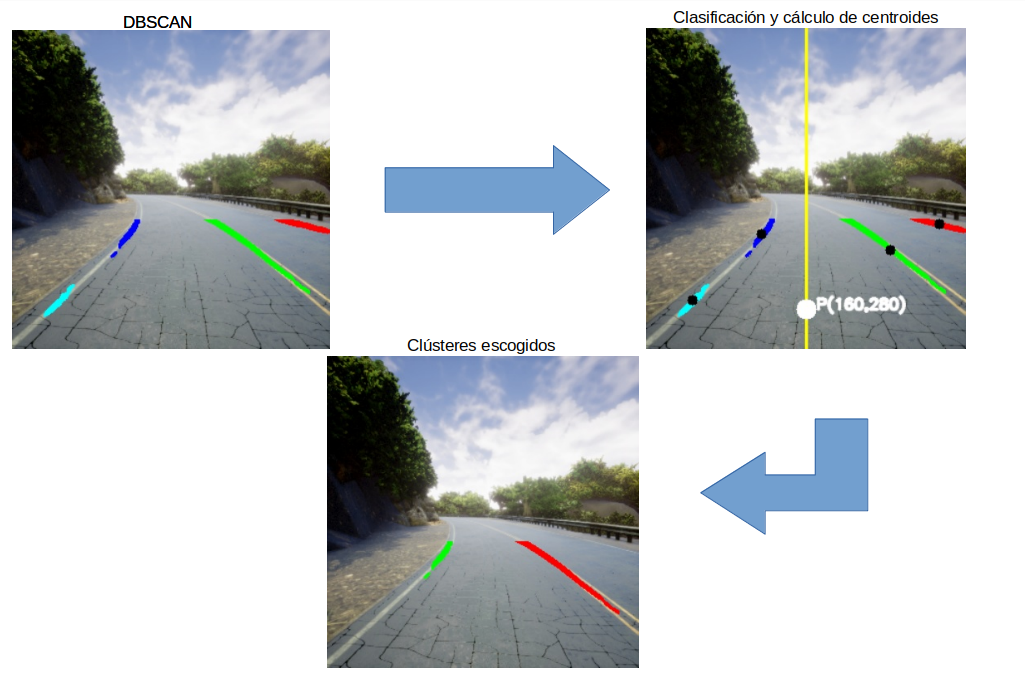
\includegraphics[scale=0.5]{figs/Diseño/DBSCAN/resultado.png}
  \end{center}
  \caption{Ilustración del proceso de elección de clústeres }
  \label{fig:DBSCAN_imagen}
\end{figure}\
Cuando tengamos el resultado de los clusters de la derecha e izquierda escogidos procederemos a realizar dos regresiones cuadráticas para construir las lineas del carril que queremos seguir.
\subsection{Regresión cuadrática}
\label{sec:Regresión cuadrática}
Como anteriormente hemos mencionado, cuando tengamos los clústeres escogidos correctamente daremos pie a la construcción de dos regresiones cuadráticas. \newline 

La regresión es un método de aprendizaje supervisado el cual consiste en aproximar un número N de puntos a una recta, curva, etc, en nuestro caso hemos escogido realizar una regresión cuadrática ya que el recorrido
que vamos a realizar las lineas detectadas por la red neuronal no son totalmente rectas si no que se tratan de lineas curvilíneas por lo que la regresión cuadrática en este papel puede 
funcionar perfectamente. 
Para la construcción de las regresiones cuadráticas utilizaremos las funciones de la libreria Numpy denominada Polyfit\footnote{\url{https://numpy.org/doc/stable/reference/generated/numpy.polyfit.html}}
y Polyval\footnote{\url{ https://numpy.org/doc/stable/reference/generated/numpy.polyval.html}}. 
Polyfit es una función que calcula los  coeficientes del polinomio que mejor se ajusta a los datos utilizando el método de los mínimos 
cuadrados para la ecuación cuadrática,obtendremos tres coeficientes, denominados a,b y c. \newline
\newline
Con dichos coeficientes realizaremos una media de los últimos diez valores y por cada cinco iteraciones dicha media se volverá a calcular, este paso lo realizamos ya que 
queremos disminuir las oscilaciones causadas de las detencciones de la red neuronal. Una vez calculados los coeficientes, realizaremos la regresión cuadrática mediante la función Polyval, dicha función calcula
la función cuadrática con los coeficientes calculados anteriormente. \newline 
Cuando obtengamos los valores de la función cuadrática, realizaremos una clasificación para quedarnos con los puntos obtenidos
de dicha función los que se encuentren en el eje y entre los valores 0 a 319, esto se debe hacer ya que dicha función como resultado puede dar numeros negativos realizando dicha regresión y en una 
imagen no se trabaja con números negativos, lo cual habrá que seleccionar los puntos correspondientes donde se encuentran en la imagen para poder seleccionarlos \newline

\begin{code}[H]
  \begin{lstlisting}[language=Python]
    def calculate_cuadratic_regression(self,points_cluster,cv_image):

    FACTOR_PIXEL = 20
    MIN_VALUE_X = (cv_image.shape[1] // 2) + FACTOR_PIXEL
    MAX_VALUE_X = cv_image.shape[1]
  
    valuesX = np.arange(MIN_VALUE_X,MAX_VALUE_X) 
    point = np.array([cv_image.shape[1]/1.104,cv_image.shape[1]])
    line = None
    extrem_point_line = None
    a = 0
    b = 0
    c = 0

    points_cluster = np.vstack((points_cluster,point))
    coefficients = np.polyfit(points_cluster[:,0],points_cluster[:,1],2)

    self.list_coeff_a.append(coefficients[0])
    self.list_coeff_b.append(coefficients[1])
    self.list_coeff_c.append(coefficients[2])

    a = np.mean(self.list_right_coeff_a[-10:])
    b = np.mean(self.list_right_coeff_b[-10:])
    c = np.mean(self.list_right_coeff_c[-10:])

    mean_coeff = np.array([a,b,c])

    self.counter_it_right += 1

    if(self.counter_it_right  > 5):
      self.list_right_coeff_a.clear()
      self.list_right_coeff_b.clear()
      self.list_right_coeff_c.clear()  


    values_fy = np.polyval(mean_coeff,valuesX).astype(int)
    fitLine_filtered = [(x, y) for x, y in zip(valuesX, values_fy) if 0 <= y <= (cvimage.shape[1] - 1)]
    line = np.array(fitLine_filtered)
     
    return line

  \end{lstlisting}
  \caption[Función del cálculo de la regresión cuadrática]{Función del cálculo de la regresión cuadrática}
  \label{cod:codejemplo}
  \end{code}  

Este proceso se realizará dos veces, una regresión cuadrática para el grupo de clústeres detectados escogidos de la derecha y otra regresión cuadrática para el grupo de clústeres detectados
escogidos de la izquierda. \newline
Finalmente, con dichas regresiones cuadráticas se realizará una dilatación de los puntos para tener un resultado más llamativo y visual al poder
ver las regresiones cuadráticas.\newline

\begin{code}[h]
  \begin{lstlisting}[language=Python]
    def dilate_lines(self,left_line_points,right_line_points):


    img_left_line = np.zeros((WIDTH, HEIGH), dtype=np.uint8)
    img_right_line = np.zeros((WIDTH, HEIGH), dtype=np.uint8)

    img_left_line[left_line_points[:,0],left_line_points[:,1]] = 255
    img_right_line[right_line_points[:,0],right_line_points[:,1]] = 255

    
    img_left_line_dilatada = binary_dilation(img_left_line, structure=self.kernel)
    img_left_line_dilatada = (img_left_line_dilatada).astype(np.uint8)

    img_right_line_dilatada = binary_dilation(img_right_line, structure=self.kernel)
    img_right_line_dilatada = (img_right_line_dilatada).astype(np.uint8)


    return img_left_line_dilatada,img_right_line_dilatada

  \end{lstlisting}
  \caption[Función de dilatación de los puntos de las regresiones]{Función de dilatación de los puntos de las regresiones}
  \label{cod:codejemplo}
  \end{code}  

\begin{figure} [H]
  \begin{center}
    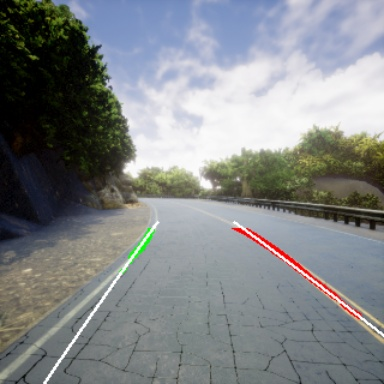
\includegraphics[scale=0.4]{figs/Diseño/Regresiones/regresion.jpg}
  \end{center}
  \caption{Resultado de la regresión cuadrática}
  \label{fig:regresión cuadrática}
\end{figure}\

\subsection{Interpolación y cálculo del centro de masas del carril}
\label{sec:Interpolación y cálculo del centro de masas del carril}

Para poder saber qué puntos se encuentran dentro de ambas regresiones cuadráticas, realizaremos una interpolación. La interpolación consiste en recorrer
los puntos de la imagen original y quedarnos con los puntos que se encuentren dentro de los límites de ambas regresiones. Se realizará dos interpolaciones, una interpolación para los puntos de la derecha
y otra interpolación para los puntos de la izquierda, estas funciones interpolan los valores de y en función de los valores de x se evaluará los valores de las puntos que se encuentren entre 
ambas regresiones cuadráticas. Cuando realizemos dicha evaluación realizaremos un filtro para seleccionar el rango de puntos que representar un fragmento del carril de color azul en la imagen
final.\newline

\begin{code}[h]
  \begin{lstlisting}[language=Python]

    def interpolate_lines(self,cvimage,points_line_left,points_line_right):


    gray_image = cv2.cvtColor(cvimage, cv2.COLOR_BGR2GRAY) 

    np_gray = np.array(gray_image)

    x, y = np.nonzero(np_gray)


    img_points = np.column_stack((x, y))

    f1 = interp1d(points_line_left[:, 0], points_line_left[:, 1],kind='slinear',fill_value="extrapolate")
    f2 = interp1d(points_line_right[:, 0], points_line_right[:, 1],kind='slinear',fill_value="extrapolate") 
    y_values_f1 = f1(img_points[:, 0])
    y_values_f2 = f2(img_points[:, 0])
    indices = np.where((y_values_f1 < img_points[:, 1]) & (img_points[:, 1] <= y_values_f2))
    
    
    points_between_lines = img_points[indices]
    filtered_points_between_lines = points_between_lines[points_between_lines[:,0] > 180]
    return filtered_points_between_lines
    

  \end{lstlisting}
  \caption[Método de interpolación]{Método del cálculo de las funciones de interpolación}
  \label{cod:codejemplo}
  \end{code}  

  \begin{figure} [H]
    \begin{center}
      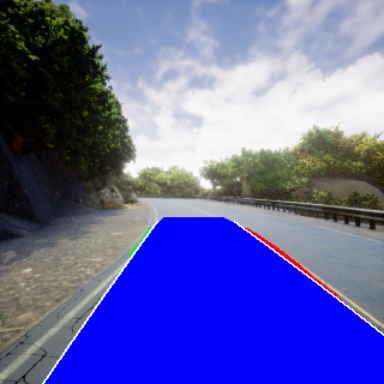
\includegraphics[scale= 0.4]{figs/Diseño/Regresiones/interpolacion.jpg}
    \end{center}
    \caption{Resultado de la interpolación}
    \label{fig:interpolación}
  \end{figure}\

  Finalmente, cuando obtengamos el cálculo del carril que queremos seguir solamente faltará calcular el centro de masas de dicho fragmento conocido como el centroide siguiendo la ecuación
  del cálculo de centro de masas de una superficie. \newline

  \begin{equation} 
    \vec{r}_{CM} = \frac{\sum_{i}m_{i} \vec{r}_{i}}{\sum_{i}m_{i}} = \frac{\sum_{i}m_{i} \vec{r}_{i}}{M} 
    \newline
  \end{equation} 
 
  Supondremos que todos los puntos tienen la misma masa (m\_i = 1). Esto simplifica el cálculo, pero en aplicaciones del mundo real, las masas pueden variar.
  El segundo paso será el calculo de la masa total, se calcula multiplicando la masa individual (m\_i) por la cantidad de puntos en el carril. A continuación calcularemos
  la suma de las posiciones de los puntos ponderadas por su masa y dividimos por la masa total calculada anteriormente. El resultado es una centro de masas conocido como centroide
  con coordenada x e y. 

  \begin{figure} [H]
    \begin{center}
      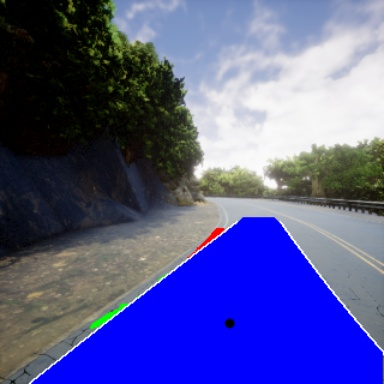
\includegraphics[scale=0.6]{figs/Diseño/Regresiones/percepcion.jpg}
    \end{center}
    \caption{Resultado del centro de masas}
    \label{fig:centro de masas}
  \end{figure}\

  Finalmente, realizamos un analisis de tiempos de cada parte para saber cuánto tiempo tarda en realizarse la percepción completa. Dicho análisis se llama profiling, con esta técnica 
  nos ayuda ver el rendimiento que podemos llegar a tener análisis global del algoritmo de percepción en cuanto a eficiencia. En la fígura , se nuestra cuanto tarda cada parte que compone 
  la percepción en segundos.

  \begin{figure} [H]
    \begin{center}
      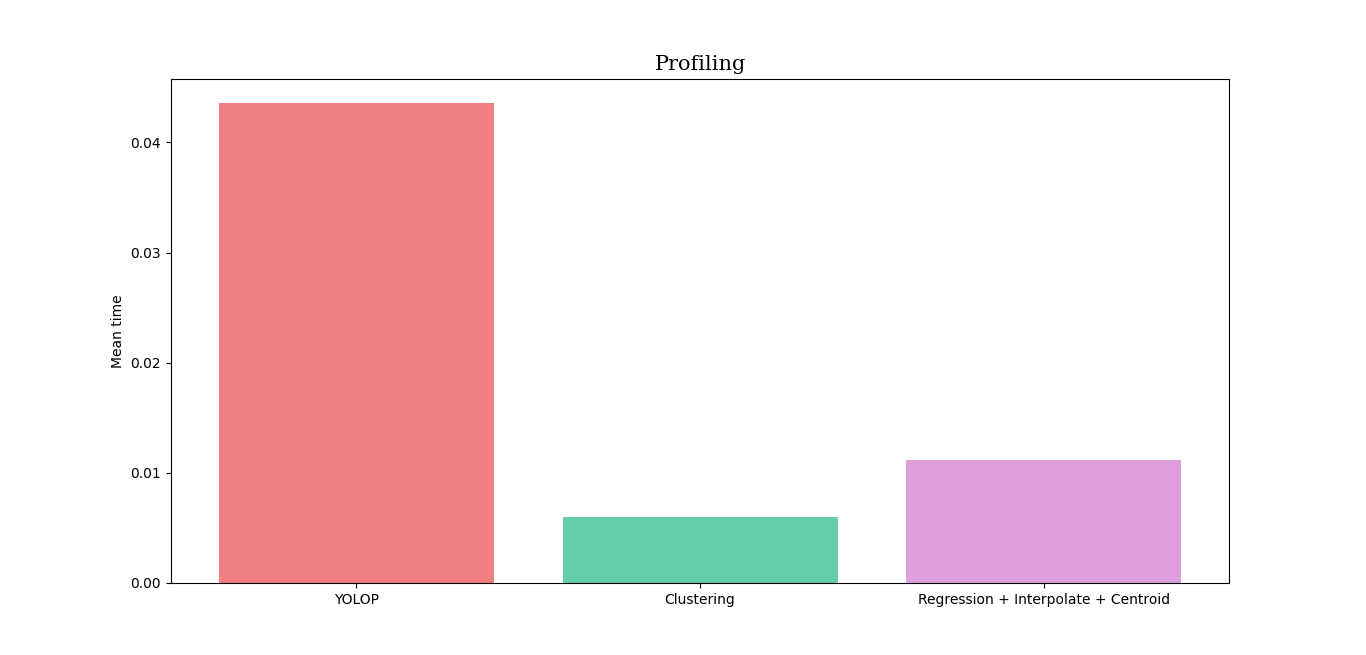
\includegraphics[scale=0.4]{figs/Diseño/Percepcion/time_profiling.png}
    \end{center}
    \caption{Profiling de las partes de la percepción}
    \label{fig:centro de masas}
  \end{figure}\

  Como podemos apreciar, la parte de la percepción que tarda más es la inferencia del modelo de YOLOP siendo el siguiente la parte de clustering utilizando el algoritmo de 

  \section{Seguimiento del carril mediante control clásico}
  \label{sec:Control}

  Una vez realizado el comportamiento de la percepción, construiremos un comportamiento autónomo con el dron basandonos en un simple controlador PID. 
 Con este primer comportamiento queremos demostrar la funcionalidad de la percepción utilizando un controlador de movimiento sencillo. \newline

 Un controlador PID (proporcional, derivativo e integral) es un 
  es un sistema que es capaz de mantener una variable (como la temperatura, velocidad o posición) cercana a un valor deseado o de referencia. Cada componente de un controlador tiene un papel 
  importante,
  la componente P (proporcional) ajusta la salida del controlador en función de la diferencia entre el valor medido y el valor deseado. 
  Cuanto mayor sea esta diferencia (error), mayor será la corrección aplicada. Sin embargo, el control proporcional solo no puede eliminar completamente el error por ello se utiliza
  las componentes derivativa e integral. La componente D (derivativa) considera la tasa de cambio del error,
  si el error cambia rápidamente, el término derivativo aplicará una corrección para evitar oscilaciones o inestabilidad.
  Con el término integral acumula el error a lo largo del tiempo y ajusta la salida del controlador en función de esta acumulación. 
  Ayuda a eliminar el error persistente o constante. Si el error es pequeño pero persistente, el término integral lo corregirá gradualmente.
  \newline

  Lo cual con este controlador PID sencillo controlaremos las velocidades respecto al error que se produce entre posición deseada y la que obtenemos. La variable deseada para estar alineados con el carril escogeremos 
  en el eje de las x el valor central de la imagen, ya que queremos en todo momento permanecer centrales, para calcular el error realizaremos la diferencia del valor deseado que seria 
  el valor central de la imagen y el valor del centroide del carril mencionado en la sección \ref{sec:Interpolación y cálculo del centro de masas del carril}. 
  A parte de este controlador, utilizaremos un pequeño controlador PD para controlar la altura del vehículo y tengamos una altura medianamente constante.Para saber a que altitud nos encontramos utilizaremos el sensor del Lidar. \newline

  Para encontrar las valores de cada término que compone ambos controladores se ha realizado a base de experimentación, empezando de manera creciente, es decir, primero utilizariamos
  la componente proporcional para ver su comportamiento, una vez que tengamos el valor del término proporcional pasaremos al termino derivativo para suavizar los movimientos que puede
  producir este término y por último utilizariamos la parte integral para eliminar el error. El controlador PID se usará para controlar la velocidad de giro del dron en cuanto a la velocidad lineal. \newline
  tendremos un valor constante. 

  \begin{code}[h]
    \begin{lstlisting}[language=Python]

      kp_height = 0.1
      kd_height = 0.4

      kp_speed_controller = 0.09
      kd_speed_controller = 0.1
      ki_speed_controller = 0.008
     
    \end{lstlisting}
    \caption[Valores de las variables del PD del control de altura y del PID del controlador de velocidad angular]{Valores de las variables del PD del control de altura y del PID del controlador de velocidad angular}
    \label{cod:codejemplo}
    \end{code} 

  \section{Seguimiento del carril mediante aprendizaje por refuerzo}
  \label{sec:Reinforcement learning}

  Como mencionamos en la sección \ref{sec:IA},el aprendizaje por refuerzo consiste en enseñar un agente 
  desempeñar un comportamiento mediante recompensas y penalizaciones. Este comportamiento se aprende a base de interacciones con el entorno de trabajo y observaciones de como puede responder,
  de forma similar a los niños que exploran el mundo que les rodea y aprenden las acciones que les ayudan a alcanzar un objetivo. Se compone de diferentes elementos claves:
  \begin{itemize} 
    \item \textbf{Agente}: El agente es una entidad o modelo que pretendemos entrenar para que aprenda a tomar decisiones (acciones) en función del estado en el que nos encontremos. Nuestro 
    agente será el dron.
    \item \textbf{Entorno}: Ambiente en donde interactua el agente para que pueda aprendar el comportamiento deseado. El dron estará interectuando sobre el entorno de Coastline que nos proporciona Airsim 
    durante las fases de pruebas. 
    \begin{figure} [H]
      \begin{center}
        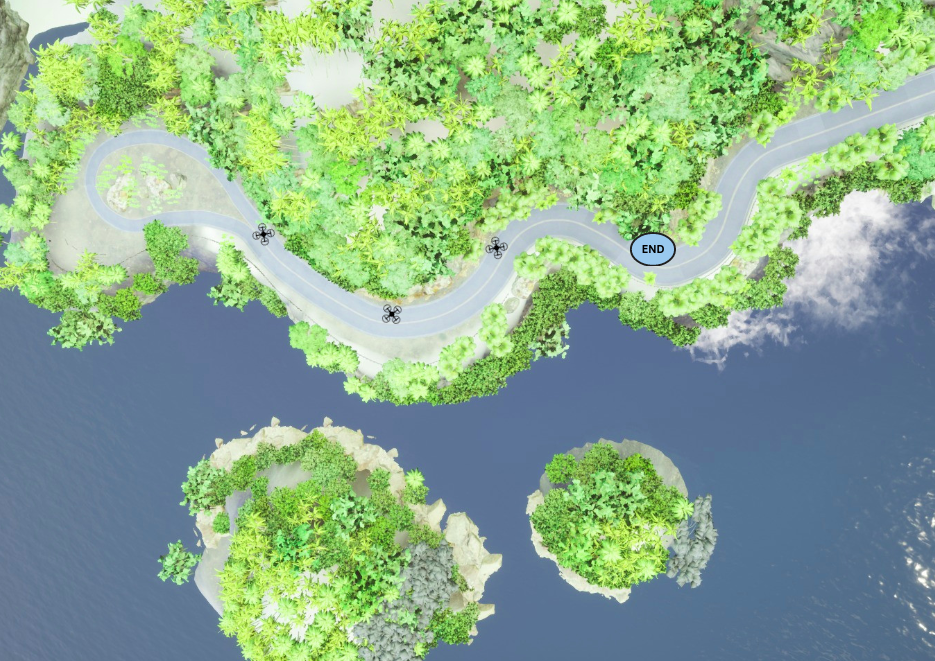
\includegraphics[scale=0.5]{figs/Diseño/RL/entorno.png}
      \end{center}
      \caption{Entorno en la fase de entrenamiento del sigue carril basado en Q-Leaning}
      \label{fig:Entorno}
    \end{figure}\

    Dentro de este circuito, hemos escogido tres localizaciones distintas para el vehículo a la hora de realizar el entrenamiento con el algoritmo de QLearning. Como se puede apreciar en la figura \ref{fig:Entorno} las posiciones
    tienen una distancia entre ellas considerablemente. 
    \item \textbf{Estados}: Condiciones en las que se puede encontrar el agente en ese instante de tiempo. Para la definición de los estados, dividiremos la imagen que damos como la salida de la detencción del carril en 14 franjas, dichas franjas tendrán una 
    separación de 10 pixeles. Las franjas representarán cada estado en el que se puede encontrar el agente.Empezaremos a definir el primer estado desde la izquierda hasta la derecha
    hasta conseguir los 14 estados correspondientes, 7 estados izquierda, 1 estado central y 6 estados derecha. 
    \item \textbf{Acciones}: Movimientos que puede realizar el agente dentro del estado en el entorno de entrenamiento.Tendremos en total 21 acciones que podrá escoger el agente en el algoritmo de Q-Learning, se componen de pares de velocidades lineales y angulares. Las velocidades lineales
    tendrán un intervalo de 0.1 m/s hasta 2.0 m/s, así siendo el intervalo de la velocidad angular de -25 hasta 25 grados/segundo, teniendo giros hacia la izquierda y hacia la derecha. Dichos pares
    de velocidades serán formados a partir de la función que nos proporciona Numpy llamada linspace\footnote{\url{https://numpy.org/doc/stable/reference/generated/numpy.linspace.html}}. \newline
  
    \begin{code}[h]
      \begin{lstlisting}[language=Python]
  
        
        def build_actions():
            ACTIONS = []
            speeds_actions = np.linspace(0.1,2.0,11, dtype=float)
            angular_speeds = np.linspace(-25,25, 21)
        
            left_angular_speeds = angular_speeds[:10]
            right_angular_speeds = np.flip(angular_speeds[-10:])
            central_angular_speed = angular_speeds[10]
            speeds = speeds_actions[:10]
            central_speed = speeds_actions[10]
        
            for i in range(len(speeds)):
                ACTIONS.append([round(speeds[i],3),round(left_angular_speeds[i],3)])
        
            ACTIONS.append([round(central_speed,3),0.0])
        
            for  i in reversed (range(len(speeds))):
                ACTIONS.append([round(speeds[i],3),round(right_angular_speeds[i],3)])
  
            return ACTIONS
       
      \end{lstlisting}
      \caption[Construcción de las acciones para Q-Learning]{Construcción de las acciones para Q-Learning}
      \label{cod:codejemplo}
      \end{code}
      
    \item \textbf{Función de Recompensa o Penalizaciones}: Consiste en como queremos premiar o penalizar al agente con el objetivo que queremos cumplir. Las recompensas o penalizaciones se recogen
    en una función, dicha función es independiente en cada diseño del objetivo que quiere completar el agente. La función de recompensa constará de dos partes premiando al dron de que se 
    permanezca centrado en el carril y además preamiarle por mantener una orientación adecuada respecto al carril, asegurando que se navegue de forma paralela al mismo. Tanto la recompensa por 
    mantenerse centrado en el carril como la orientación respecto al carril será normalizada entre valores de 0-, penalizando con un valor constante al dron cuando se salga del carril o 
    se pierda la percepción. La implementación de la función de recompensa y las penalizaciones se puede ver el siguiente código:

    \begin{code}[H]
      \begin{lstlisting}[language=Python]
  
        def reward_function(self,cx,angle):

        reward = 0
        target_heading = 0
        error_lane_center = (WIDTH/2 - cx)
        heading_difference = (target_heading - angle) 
        
        MIN_ERROR = 0
        MAX_ERROR = 80

        MIN_ANGLE = 0
        MAX_ANGLE = 70

        CENTRE_WEIGHT = 0.85
        ANGLE_WEIGHT = 0.15
        
        if (self.is_exit_lane(cx)):
            
            reward = -10

        else:

            
            normalise_error_centre = (abs(error_lane_center) - MIN_ERROR) / (MAX_ERROR - MIN_ERROR)
            reward_centre = 1 - normalise_error_centre

            
            normalise_error_angle = (abs(heading_difference) - MIN_ANGLE) / (MAX_ANGLE - MIN_ANGLE)
            reward_angle = 1 - normalise_error_angle


            reward = (reward_centre * CENTRE_WEIGHT) + (reward_angle * ANGLE_WEIGHT)
            
        return reward
       
      \end{lstlisting}
      \caption[Función de recompensa]{Función de recompensa}
      \label{cod:codejemplo}
      \end{code}
    \item \textbf{Política}: Determina que acción realizar en cada estado que se encuentre el agente. Dicha política varía según el tipo de algoritmo que queremos seguir dentro de Reinforcement learning.
    Puede ser determinista o estocástica. \newline

    Seguiremos la política epsilon-greedy\cite{Epsilon-greedy}, que consiste 
 equilibrar la exploración y explotación en la fase de entrenamiento. Cuando el agente tenga que escoger la acción que tomar tendra en cuenta dos enfoques:
 
 \begin{itemize}
   \item Exploración (con probabilidad $\epsilon$): El agente escogerá una acción al azar para explorar
   \item Explotación(con probabilidad $ 1 - \epsilon$): El agente escogerá la acción con el valor de la tabla Q(S,A) más alto, es decir, la mejor acción conocida
 \end{itemize}
 
 El parámetro $\epsilon$ es el responsable de controlar la proporción de exploración frente a explotación, si $\epsilon$  es alto el agente explorará más en cambio si $\epsilon$ es bajo
 el agente se centrará en la explotación. Por lo que en la elección de acción se generará un numero n aleatoriamente, si n es menor que la probabilidad $\epsilon$ la acción se escogerá aleatoriamente
 en cambio si n es mayor que la probabilidad de $\epsilon$ la acción será que mayor valor tenga en la tabla Q(S,A) para dicho estado. \newline
 
 Dentro de esta política la probabilidad de $\epsilon$ será decayente, es decir, no ser un valor constante en cada episodio que nos encontremos, lo que realizaremos sera una disminuición 
 de esta probabilidad para conseguir que el agente con el paso del tiempo poco a poco explote lo que ha aprendido y que el modelo llegue a una convergencia óptima. Para llevar a cabo el descenso
 de $\epsilon$ se puede realizar de varias formas, por ejemplo podemos realizarlo linealmente, logaritmicamente, exponencial o escalonado. \newline
  \end{itemize}

  El algoritmo Q-Learning  se basa en seguir una función acción-recompensa formada por un tabla estado-acción la cual iremos rellenando siguiendo la siguiente ecuación
  de Bellman\cite{Bellman}:
  
  \begin{equation} 
    Q(s, a) = Q(s, a) + \alpha \cdot [R(s, a) + \gamma \cdot \max Q(s', a') - Q(s, a)]
  \end{equation} 

  en donde, 

  \begin{itemize}
    \item \textbf{$Q(s, a)$}: Valor Q para el estado $s$ y la acción $a$. Se trata de una matriz formada por estado y acción.
    \item \textbf{$\alpha$}: Tasa de aprendizaje entre un valor de 0 a 1. Consiste en el porcentaje que daremos al agente para el proceso de aprendizaje, si dicho valor es alto daremos más peso al valor aprendido 
    \item \textbf{$R(s, a)$}: Recompensa por tomar la acción $a$ en el estado $s$. La función de recompensa es crucial en el proceso de aprendizaje del agente, evalua como es favorable o deseable
    es una acción tomada por el agente en el estado que se encuentre. Proporciona información al agente sobre que acciones maximizan la recompensa total a lo largo del tiempo. Dicha función
    de recompensa es diseñada dependiendo de cual sea el objetivo de tu agente. 
    \item \textbf{$\gamma$}: Factor de descuento entre un valor de 0 a 1. Modela la importancia de las recompensas futuras en relación con las recompensas inmediatas, refleja la importancia del agente
    por las recompensas a largo plazo. Un valor alto sifnigicará que le agente valorará mucho las recompensas futuras, mientras que un valor bajo indica que se enfocará más en las recompensas
    inmediatas
    \item \textbf{$\max Q(s', a')$}: Valor Q máximo en el próximo estado $s'$ para todas las acciones posibles $a'$.
\end{itemize}

A la medida que vayamos avanzando en la fase de entrenamiento, iremos rellenando la tabla Q(s,a) para más adelante indexar en ella en la fase de inferencia

\subsubsection{Fase de entrenamiento}
\label{sec:fases_ql}
 Antes de adentrarnos en esta fase, definiremos dos conceptos importantes:
 \begin{itemize}
  \item \textbf{Episodios}: Se define episodio como una secuencia completa de interacciones que se produce entre el agente y el entorno. Cada episodio comienza con un estado inicial y consta de una serie 
  de pasos o acciones tomadas por el agente.
  \item \textbf{Iteraciones (steps)}: Son los pasos que puede dar un agente en el entorno dentro de un episodio. Estos pasos pueden incluir observaciones del entorno, decisiones tomadas por el agente
  y las consecuentes recompensas o penalizaciones recibidas.
\end{itemize}

 
 La fase de entrenamiento consiste en el que el agente explore todo lo máximo posible en el entorno respecto a los estados que tiene y las acciones que puede tomar, es decir, al comienzo del entrenamiento se inicializará la tabla Q(S,A) a cero todos sus valores, esta representación
 al comienzo es así ya que el agente desconoce por completo el entorno hasta que poco a poco vaya iterando sobre el en cada estado tomando x accion. \newline
 
 Basicamente, en cada iteración del algoritmo se escogerá una acción según si estamos en exploración o explotación, se calculará la recompensa obtenida e iteraremos de nuevo sobre el algoritmo.

 El entrenamiento finaliza cuando el agente haya aprendido el objetivo que queremos seguir, esto se sabe cuando las iteraciones del algoritmo y la recompensa acumulada del agente en esta 
 fase se estabilice y tenga valores constantes, es decir, no cambia significativamente con más iteraciones, esto se denomina que el modelo ha convergido y pasaremos a la fase de inferencia. \newline

Durante esta fase, dejamos el algoritmo de Q-Learning entrenando durante aproximadamente 12 horas. De esta manera, nos podemos asegurar que el algoritmo completará el entrenamiento de manera correcta y poco a poco 
acabará convergiendo. En las fíguras , se presentan dos gráficas respecto 


\subsubsection{Fase de inferencia}
\label{sec:fases_inferencia}
La fase de inferencia consiste en indexar la tabla Q(S,A) que hemos ido rellenando en la fase de entrenamiento. El agente cuando se encuentré en un estado especifico consultará la tabla Q(S,A) para
encontrar la mejor acción en ese estado (cuando mencionamos la mejor acción nos referimos al máximo valor en la tabla que tenga en ese estado). Cuando el agente tome dicha acción se moverá al siguiente estado
siendo así un proceso iterativo hasta alcanzar la meta. En esta fase, los valores de la tabla permanecen constantes y se utiliza para la toma de decisiones basadas en el conocimiento
aprendido en la fase de entrenamiento. 








  


  




  














        


  

